% tlmgr install ...
\documentclass{article}
\usepackage{graphicx} % Required for inserting images
\usepackage{wrapfig}
\usepackage{amsmath} % Required for some math elements
\usepackage{mathtools} % Required for \coloneqq command
\usepackage[margin=2cm]{geometry} % Set margins to 2cm
\usepackage[danish]{babel} % Set language to Danish
\usepackage{tocloft}
\usepackage{cancel}
\usepackage{csquotes}
\usepackage{xcolor}
\usepackage{nicematrix}
\usepackage{caption}
\usepackage{minted}
\usepackage{pdfpages}
\usemintedstyle{vs}
\setminted{breaklines, frame=lines, linenos, fontsize=\small}

\newenvironment{code}{\captionsetup{type=listing}}{}


\captionsetup{font=footnotesize}



% Define a custom color
\definecolor{backcolour}{rgb}{0.95,0.95,0.92}
\definecolor{codegreen}{rgb}{0,0.6,0}

% Required package
\usepackage{tikz}
\usetikzlibrary{positioning}

% Input layer neurons' number
\newcommand{\inputnum}{3} 

% Hidden layer neurons' number
\newcommand{\hiddennum}{5}  

% Output layer neurons' number
\newcommand{\outputnum}{2} 

\usepackage[
  style=apa,
  sortcites=true,
  sorting=nyt,
  backend=biber,
  autocite=inline
]{biblatex}
\addbibresource{paper.bib}

\renewcommand\cftsecfont{\normalfont}
\renewcommand{\cftsecleader}{\cftdotfill{\cftsecdotsep}}
\renewcommand\cftsecdotsep{\cftdot}
\renewcommand\cftsubsecdotsep{\cftdot}
\renewcommand\cftsubsubsecdotsep{\cftdot}


% fig ref
\newcommand{\figureref}[1]{(Figur \ref{#1})}

% listing ref 
\newcommand{\listingref}[1]{(Kodestykke \ref{#1})}

\newcommand\Ccancel[2][black]{
    \let\OldcancelColor\CancelColor
    \renewcommand\CancelColor{\color{#1}}
    \cancel{#2}
    \renewcommand\CancelColor{\OldcancelColor}
}

\captionsetup[listing]{name=Kodestykke}


\makeatletter
\newcommand{\subject}[1]{\gdef\@subject{#1}}
\newcommand{\class}[1]{\gdef\@class{#1}}
\newcommand{\mentor}[1]{\gdef\@mentor{#1}}
\renewcommand{\maketitle}{\bgroup\setlength{\parindent}{0pt}
\begin{flushleft}
  \textbf{\@title}
  \rule{\textwidth}{0.2pt}\\\vspace{0.2em}
  \huge{
    Genkendelse af håndskrevne tal med neurale netværk
  }\\\vspace{1em}
  % normal text
  \normalsize
  \@subject\\\vspace{1em}
  \@author\\
  \@class\\
  \@date\\\vspace{1em}
  Vejledere:\\\@mentor
\end{flushleft}\egroup
}
\makeatother

\title{\Huge{Studie Område Projekt}}
\subject{Matematik A / Programmering B}
\author{Victor Østergaard Nielsen}
\class{3di - H. C. Ørsted Gymnasiet Lyngby}
\date{15/12/2024}
\mentor{Jan Strauss Hansen (Matematik A) \\ Kristian Krabbe Møller (Programmering B)}

\begin{document}
\thispagestyle{empty}
\includepdf[pages=-]{Victor+Østergaard+Nielsen_3di.pdf}

\maketitle
\vspace{3cm}
\begin{center}
  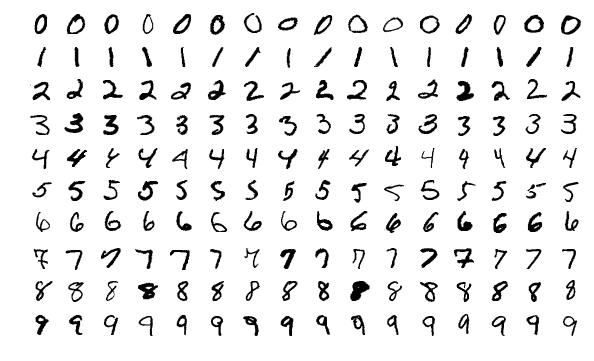
\includegraphics[width=0.7\textwidth]{MNIST3.jpg}
  \captionof{figure}{Eksempel fra MNIST-datasættet \parencite{LeCun_1994,delclos2021computer}}
\end{center}
\thispagestyle{empty}
\newpage

\section*{Resumé}
Denne opgave er bestående af 15,5 normalsider og 4 sider med symboltegn, total: 19,5 sider.\\\\
Denne opgave undersøger, hvordan et simpelt neuralt netværk kan implementeres uden unødvendige abstraktioner eller biblioteker for at genkende håndskrevne tal i realtid på en digital tegneflade. Formålet er at afdække de matematiske og teknologiske principper bag neurale netværk, herunder matrixregning og gradient descent algoritmen, og at vurdere deres effektivitet som løsning til denne specifikke udfordring. Analysen viser, at neurale netværk kan lære at genkende mønstre ved hjælp af træningsdata og optimeringsalgoritmer. Opgaven demonstrerer, hvordan et netværk med input-, skjulte- og outputlag kan programmeres i Python, og hvordan der kan bruges aktiveringsfunktioner som sigmoid og softmax til at beskrive ikke-linearitet samt repensentere en sandsynlighedsfordeling. Konklusionen peger på, at neurale netværk, selv i en simpel udgave, er en effektiv og nogenlunde fleksibel løsning til genkendelsen af håndskrevne tal i realtid. Samtidig erkendes det, at mere avancerede netværk som convolutional neural networks (CNNs) kan tilbyde bedre præcision, men også kræver større beregningskraft og kompleksitet.
\newpage

\tableofcontents
\newpage
\pagenumbering{arabic} 

\section{Indledning}
I takt med, at kunstig intelligens får en større rolle i vores hverdag, rejser det mange fundamentale spørgsmål, heriblandt: Hvordan man kan optimere maskiners evne til at forstå og tolke menneskelige input? Denne opgave fokuserer på udviklingen af et simpelt neuralt netværk, der kan genkende håndskrevne tal i realtid gennem en digital tegneflade. Problemstillingen er spændende, fordi den kombinerer matematik og programmering for at simulere hjernens måde at lære og tilpasse sig på. Det er et emne, der både har stor relevans inden for uddannelse og teknologi. I en tid, hvor automatisering og dataforståelse er afgørende for innovation, er det vigtigt at forstå, hvordan neurale netværk kan bruges til at efterligne menneskets evne til at genkende mønstre. Specifikt undersøger denne opgave, hvordan et neuralt netværk kan implementeres uden brug af avancerede biblioteker eller unødvendige abstraktioner, og hvordan matematiske principper som matrixregning og gradient descent spiller en central rolle i træningen og optimeringen af netværket. Problemstillingen knytter sig direkte til praksis ved at tage udgangspunkt i en konkret anvendelse, nemlig genkendelse af håndskrevne tal, som kan bruges i applikationer såsom OCR-systemer og andre klassifikationsopgaver. Opgaven fokuserer dog bevidst på en simplificeret model for at holde analysen fokuseret og anvendelig. Mere avancerede teknologier såsom convolutional neural networks (CNNs) inddrages ikke, da målet er at demonstrere forståelsen af grundprincipperne bag neurale netværk og deres implementering. Læseren kan således forvente en praktisk og matematisk tilgang, der gør det muligt at forstå sammenhængen mellem teori og praksis i maskinlæring.

\newpage
\section{Matricer og matrixregning}
\subsection{Matricer}
En matrice er en tabel af tal, der er arrangeret i rækker og kolonner. En matrice kan repræsenteres med et stort bogstav, f.eks. $A$, og elementerne i matricen kan repræsenteres som $a_{ij}$, hvor $i$ er rækken og $j$ er kolonnen. En matrice med $m$ rækker og $n$ kolonner kaldes en $m \times n$ matrice. En matrice med lige mange rækker og kolonner kaldes en kvadratisk matrice. En matrice med kun én række kaldes en rækkevektor, og en matrice med kun én kolonne kaldes en søjlevektor. \parencite{Lauritzen_2019}\\\\
\begin{align}
  \underbrace{A = \begin{bmatrix}
    a_{11} & a_{12} & \ldots & a_{1n} \\
    a_{21} & a_{22} & \ldots & a_{2n} \\
    \vdots & \vdots & \ddots & \vdots \\
    a_{m1} & a_{m2} & \ldots & a_{mn}
  \end{bmatrix}}_{\text{$m \times n$ Matrice}} 
  &&
  \underbrace{B = \begin{bmatrix}
    b_{11} \\
    b_{21} \\
    \vdots \\
    b_{m1}
  \end{bmatrix}}_{\text{Søjlevektor}} 
  &&
  \underbrace{C = \begin{bmatrix}
    c_{11} & c_{12} & \ldots & c_{1n}
  \end{bmatrix}}_{\text{Rækkevektor}} 
\end{align}
\subsection{Matrixregning}
Matrixregning er en vigtig del af matematikken bag neurale netværk og er derfor vigtig at forstå. Der er flere forskellige operationer, der kan udføres på matricer, herunder addition, subtraktion, skalarmultiplikation og matrixmultiplikation m.m.
\subsubsection{Addition og subtraktion}
For at addere eller subtrahere to matricer skal de have samme dimensioner, altså de skal have samme mængde rækker og søjler. Givet dette, så er matmatkiken ikke meget andlernedes fra normale tal, det betyder at: $A + B = B + A$. Da de 2 matricer har samme dimension udføres addition og subtraktion således \parencite{Lauritzen_2019}:
\begin{align}
  A + B = \begin{bmatrix}
    a_{11} & a_{12} \\
    a_{21} & a_{22}
  \end{bmatrix} + \begin{bmatrix}
    b_{11} & b_{12} \\
    b_{21} & b_{22}
  \end{bmatrix} = \begin{bmatrix}
    a_{11} + b_{11} & a_{12} + b_{12} \\
    a_{21} + b_{21} & a_{22} + b_{22}
  \end{bmatrix}
\end{align}
Hver position i $A$ matricen bliver altså adderet med samme position i $B$ matricen. Samme regel gælder for subtraktion.
\subsubsection{Skalarmultiplikation af matricer}
Givet tallet $k$ kan man gange $k$ på matricen $A$ således \parencite{Lauritzen_2019}:
\begin{align}
  k \cdot A = k \cdot \begin{bmatrix}
    a_{11} & a_{12} \\
    a_{21} & a_{22}
  \end{bmatrix} = \begin{bmatrix}
    k \cdot a_{11} & k \cdot a_{12} \\
    k \cdot a_{21} & k \cdot a_{22}
  \end{bmatrix}
\end{align}
\subsubsection{Elementvis anvendelse af en funktion på matricer}
Givet en funktion $f(x)$ og en $m \times n$ matrice $A$, vil $f(A)$ være en $m \times n$ matrice, hvor $f(x)$ er blevet anvendt på hvert element i $A$ \parencite{Lauritzen_2019}:
\begin{align}
  f(A) = f \left( \begin{bmatrix}
    a_{11} & a_{12} & \ldots & a_{1n} \\
    a_{21} & a_{22} & \ldots & a_{2n} \\
    \vdots & \vdots & \ddots & \vdots \\
    a_{m1} & a_{m2} & \ldots & a_{mn}
  \end{bmatrix} \right) = \begin{bmatrix}
    f(a_{11}) & f(a_{12}) & \ldots & f(a_{1n}) \\
    f(a_{21}) & f(a_{22}) & \ldots & f(a_{2n}) \\
    \vdots & \vdots & \ddots & \vdots \\
    f(a_{m1}) & f(a_{m2}) & \ldots & f(a_{mn})
  \end{bmatrix}
\end{align} 
\subsubsection{Matrixmultiplikation}
At gange to matricer sammen er lidt mere kompliceret, det indebærer først og fremmest at de 2 matricer er af kompatibel størrelse. Hvis $A$ er en $m \times p$ matrice og $B$ er en $p \times r$ matrice, så er $C = A \cdot B$ en $m \times r$ matrice. Bemærk at antallet af kolonner i $A$ matricen skal være lig antallet af rækker i $B$ matricen. For at finde elementet $c_{ij}$ i $C$ matricen ganges række $i$ i $A$ matricen med kolonne $j$ i $B$ matricen. Dette gøres ved at gange elementerne i række $i$ i $A$ matricen med elementerne i kolonne $j$ i $B$ matricen og summere dem. F.eks. hvis $A$ er en $3 \times 2$ matrice og $B$ er en $2 \times 3$ matrice, så er $C$ en $3 \times 3$ matrice, og elementet $c_{11}$ i $C$ matricen findes således \parencite{Simonson_2015}:
\begin{align}
  c_{11} = a_{11} \cdot b_{11} + a_{12} \cdot b_{21}
\end{align}
Intuitivt kan dette visualiseres ved at tegne $A$ og $B$ matricerne således \parencite{Simonson_2015}:  
\begin{align}
  \begin{NiceMatrix} 
    & & b_{11} & b_{12} & b_{13} \\
    & & b_{21} & b_{22} & b_{23} \\[1mm]
    a_{11} & a_{12} &  &  &  \\
    a_{21} & a_{22} &  &  &  \\
    a_{31} & a_{32} &  &  &  \\
  \CodeAfter
    \SubMatrix[{1-3}{2-5}]
    \SubMatrix[{3-1}{5-2}]
    \SubMatrix[{3-3}{5-5}]
\end{NiceMatrix}
\end{align}
For at finde elementet $c_{11}$ i $C$ matricen, ganges række 1 i $A$ matricen med kolonne 1 i $B$ matricen, dette er visualiseret herunder \parencite{Simonson_2015}:
\begin{align}
  \begin{NiceMatrix} 
    & & \color{blue} b_{11} & b_{12} & b_{13} \\
    & & \color{violet} b_{21} & b_{22} & b_{23} \\[1mm]
    \color{red} a_{11} & \color{teal} a_{12} & c_{11} &  &  \\
    a_{21} & a_{22} &  &  &  \\
    a_{31} & a_{32} &  &  &  \\
  \CodeAfter
    \SubMatrix[{1-3}{2-5}]
    \SubMatrix[{3-1}{5-2}]
    \SubMatrix[{3-3}{5-5}]
\end{NiceMatrix}
&&
  c_{11} = {\color{red} a_{11}} \cdot {\color{blue} b_{11}} + {\color{teal} a_{12}} \cdot {\color{violet} b_{21}}
\end{align}
Samme operation gentages for resten af positionerne i $C$ matricen:
\begin{align}
  \begin{NiceMatrix} 
    & & b_{11} & b_{12} & b_{13} \\
    & & b_{21} & b_{22} & b_{23} \\[1mm]
    a_{11} & a_{12} & c_{11} & c_{12} & c_{13} \\
    a_{21} & a_{22} & c_{21} & c_{22} & c_{23} \\
    a_{31} & a_{32} & c_{31} & c_{32} & c_{33} \\
  \CodeAfter
    \SubMatrix[{1-3}{2-5}]
    \SubMatrix[{3-1}{5-2}]
    \SubMatrix[{3-3}{5-5}]
\end{NiceMatrix}
\end{align}
Det ses nu visuelt at den resulterende matrice $C$ er en $3 \times 3$ matrice når $A$ er en $3 \times 2$ matrice og $B$ er en $2 \times 3$ matrice. Det skal dog bemærkes at matrixmultiplikation ikke er kommutativ, altså $A \cdot B \neq B \cdot A$. Dette kan også ses visuelt ved at bytte om på $A$ og $B$ matricerne:
\begin{align}
\begin{NiceMatrix} 
    & & b_{11} & b_{12} & b_{13} \\
    & & b_{21} & b_{22} & b_{23} \\[1mm]
    a_{11} & a_{12} & c_{11} & c_{12} & c_{13} \\
    a_{21} & a_{22} & c_{21} & c_{22} & c_{23} \\
    a_{31} & a_{32} & c_{31} & c_{32} & c_{33} \\
  \CodeAfter
    \SubMatrix[{1-3}{2-5}]
    \SubMatrix[{3-1}{5-2}]
    \SubMatrix[{3-3}{5-5}]
\end{NiceMatrix}\label{eq:matrixmultiplikation1}
&&
\begin{NiceMatrix} 
    & & & a_{11} & a_{12} \\
    & & & a_{21} & a_{22} \\
    & & & a_{31} & a_{32} \\[1mm]
    b_{11} & b_{12} &  b_{13} & c_{11} & c_{12} \\
    b_{21} & b_{22} &  b_{23} & c_{21} & c_{22} \\
    \CodeAfter
    \SubMatrix[{1-4}{3-5}]
    \SubMatrix[{4-1}{5-3}]
    \SubMatrix[{4-4}{5-5}]
\end{NiceMatrix}
\end{align}
Det ses at $A \cdot B$ og $B \cdot A$ ikke er ens, og derfor er matrixmultiplikation ikke kommutativ. \parencite{Lauritzen_2019} Selv med to kvadratiske matricer af samme dimension er matrixmultiplikation ikke nødvendigvis kommutativ. Dette kan betragtes i følgende eksempel:
\begin{align}
  A = \begin{bmatrix}
    1 & 2 \\
    3 & 4
  \end{bmatrix}
  &&
  B = \begin{bmatrix}
    5 & 6 \\
    7 & 8
  \end{bmatrix}
\end{align}
\begin{align}
  A \cdot B = \begin{bmatrix}
    1 \cdot 5 + 2 \cdot 7 & 1 \cdot 6 + 2 \cdot 8 \\
    3 \cdot 5 + 4 \cdot 7 & 3 \cdot 6 + 4 \cdot 8
  \end{bmatrix} = \begin{bmatrix}
    19 & 22 \\
    43 & 50
  \end{bmatrix}
  &&
  B \cdot A = \begin{bmatrix}
    5 \cdot 1 + 6 \cdot 3 & 5 \cdot 2 + 6 \cdot 4 \\
    7 \cdot 1 + 8 \cdot 3 & 7 \cdot 2 + 8 \cdot 4
  \end{bmatrix} = \begin{bmatrix}
    23 & 34 \\
    31 & 46
  \end{bmatrix}
\end{align}
Det ses at $A \cdot B \neq B \cdot A$, matrixmultiplikation er altså ikke kommutativ, hverken i den resulterende størrelse i ikke kvadratiske matricer eller i kvadratiske matricer af samme størrelse. \parencite{Lauritzen_2019}
\subsubsection{Transponering af matricer}
Transponering af en matrice betyder at bytte om på rækker og kolonner. Hvis $A$ er en $m \times n$ matrice, så er transponeringen af $A$ en $n \times m$ matrice, og elementet $a_{ij}$ i $A$ matricen bliver til elementet $a_{ji}$ i $A^T$ matricen. Dette kan visualiseres ved at tegne $A$ matricen og $A^T$ matricen \parencite{Lauritzen_2019}:
\begin{align}
  A = \begin{bmatrix}
    a_{11} & a_{12} \\
    a_{21} & a_{22} \\
    a_{31} & a_{32}
  \end{bmatrix}
  &&
  A^T = \begin{bmatrix}
    a_{11} & a_{12} & a_{13} \\
    a_{21} & a_{22} & a_{23}
  \end{bmatrix}
\end{align}
\section{Neurale netværk}
\subsection{Introduktion}
\begin{wrapfigure}{r}{6cm}
  \vspace{-0.5cm}
  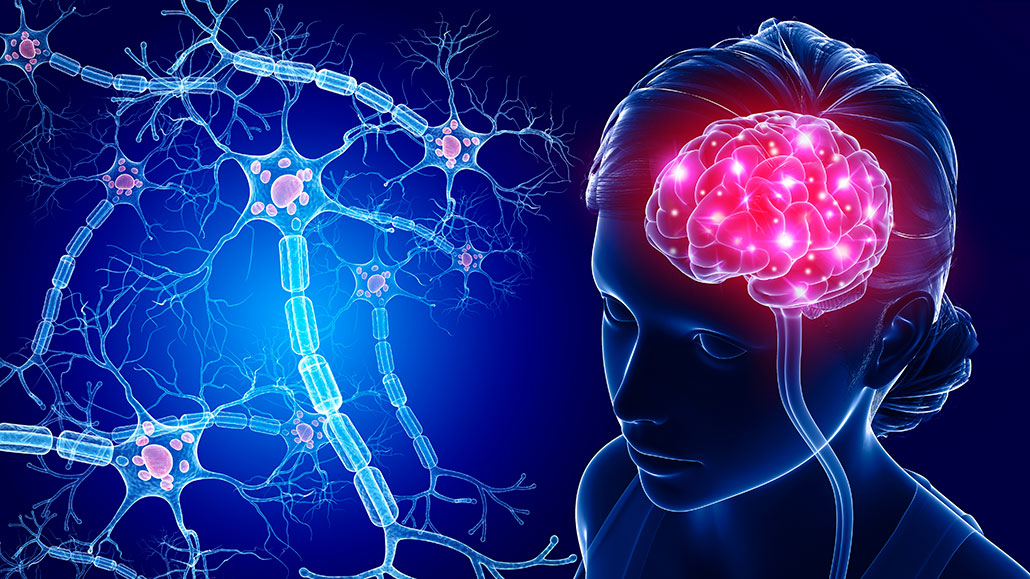
\includegraphics[width=6cm]{neurons.jpg}
  \vspace{-0.5cm}
  \caption{Neuroner i menneskehjernen fra \parencite{St_Clair_2021}}
  \label{fig:neurons}
  \vspace{0.5cm}
  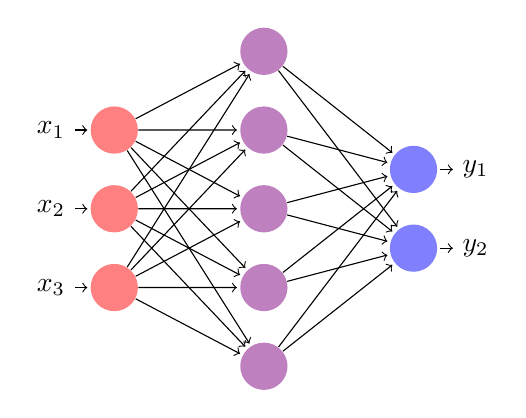
\begin{tikzpicture}

% Input Layer
\foreach \i in {1,...,\inputnum}
{
  \node[circle, 
    minimum size = 6mm,
    fill=red!50] (Input-\i) at (0,-\i) {};
}

% Hidden Layer
\foreach \i in {1,...,\hiddennum}
{
  \node[circle, 
    minimum size = 6mm,
    fill=violet!50,
    yshift=(\hiddennum-\inputnum)*5 mm
  ] (Hidden-\i) at (1.9,-\i) {};
}

% Output Layer
\foreach \i in {1,...,\outputnum}
{
  \node[circle, 
    minimum size = 6mm,
    fill=blue!50,
    yshift=(\outputnum-\inputnum)*5 mm
  ] (Output-\i) at (3.8,-\i) {};
}

% Connect neurons In-Hidden
\foreach \i in {1,...,\inputnum}
{
  \foreach \j in {1,...,\hiddennum}
  {
    \draw[->, shorten >=1pt] (Input-\i) -- (Hidden-\j);	
  }
}

% Connect neurons Hidden-Out
\foreach \i in {1,...,\hiddennum}
{
  \foreach \j in {1,...,\outputnum}
  {
    \draw[->, shorten >=1pt] (Hidden-\i) -- (Output-\j);
  }
}

% Inputs
\foreach \i in {1,...,\inputnum}
{            
  \draw[<-, shorten <=1pt] (Input-\i) -- ++(-0.5,0)
    node[left]{$x_{\i}$};
}

% Outputs
\foreach \i in {1,...,\outputnum}
{            
  \draw[->, shorten <=1pt] (Output-\i) -- ++(0.5,0)
    node[right]{$y_{\i}$};
}

\end{tikzpicture}

  \vspace{-0.5cm}
  \caption{Et simpelt neuralt netværk}
  \label{fig:neural_network}
  \vspace{0.5cm}
  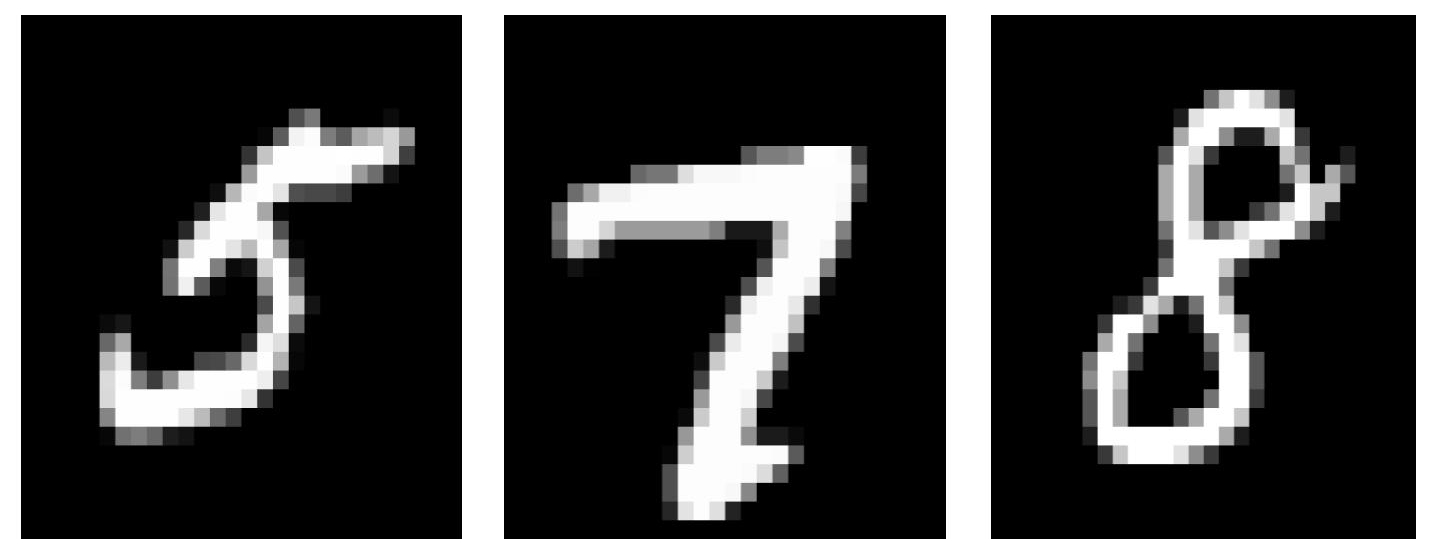
\includegraphics[width=6cm]{mnist1.jpg}
  \vspace{-0.5cm}
  \caption{Eksempel fra MNIST datasættet \parencite{LeCun_1994}}
  \label{fig:mnist}
\end{wrapfigure}
Et neuralt netværk er en matematisk model, der er inspireret af de biologiske neuroner i menneskehjernen. Et neuralt netværk består af en række lag, hvor hvert lag består af neuroner. Dette kan ses på \figureref{fig:neural_network}. Hvert neuron i et lag er forbundet til alle neuroner i det forrige lag og det næste lag. Hver forbindelse mellem neuronerne har en vægt, der bestemmer, hvor meget signalet fra det ene neuron påvirker det næste neuron. Hvert neuron har også en bias, der bestemmer, hvor let det er for neuronet at sende et signal. Et neuralt netværk består af et \color{red!90}inputlag\color{black}, et eller flere \color{violet!90}skjulte lag \color{black} og et \color{blue!90}outputlag\color{black}. Dette er illustreret på \figureref{fig:neural_network}. Denne model er altså inspireret af de mange sammenkoblede neuroner i menneskehjernen. Denne lighed er ikke tilfældig, da neurale netværk er designet til at efterligne hjernens evne til at lære. \parencite{sanderson2017neural}\vspace{5mm}\\
Bemærk \figureref{fig:mnist}. Du ved udmærket godt, hvilke tal der er på billedet, selvom du aldrig før har set netop dette 5-, 7- og 8-tal. Dette skyldes, at din hjerne er trænet til at genkende tal. Denne opgave er enormt udfordrende for et alment computerprogram, da programmet ikke har nogen intuitiv forståelse af, hvad et tal er. Den skal derfor programmeres med specifikke instruktioner for at kunne genkende tal. Denne tilgang er ikke optimal, da den kræver, at programmøren har en dyb forståelse af, hvordan tal ser ud, og hvordan de kan genkendes. Metoden er heller ikke holdbar i længden, eftersom der er uendeligt mange måder at skrive et 7-tal på. For at kunne generalisere talgenkendelse og gøre metoden mere robust overfor nye skrivemåder af tal kan neurale netværk anvendes. Antag et neuralt netværk med et tal som input og de helt rigtige vægte og biases. Denne model vil i teorien kunne genkende tal, selvom den aldrig før har set netop dette tal. Håbet er, at modellen har "lært" at generalisere træningsdataen til en mere overordnet forståelse af tal. Modellens output vil derfor være en søjlevektor med sandsynligheder for, at inputtet er et tal fra 0 til 9. Modellens prediktering vil være det tal, der har den højeste sandsynlighed ifølge modellen. \parencite{sanderson2017neural}
\clearpage
\subsection{Feedforward}
Når modellen skal prediktere, altså gå fra input til output, kaldes dette for \textit{feedforward}. Her sendes inputtet gennem alle lagene i modellen og bliver påvirket af vægtene mellem neuronerne samt biaset i hvert neuron. Herunder ses et simpelt neuralt netværk med kun 1 neuron i hvert lag og et skjult lag, hvor $a_n$ er aktiveringen af neuronen i lag $n$, og $w_n$ er vægten mellem neuronen i lag $n$ og lag $n+1$ \parencite{sanderson2017neural}:
\begin{center}
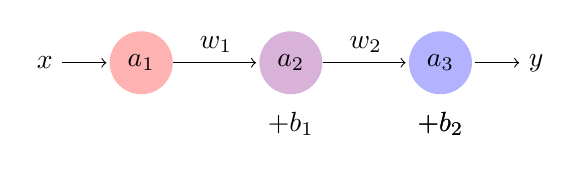
\begin{tikzpicture}
  \node[circle, minimum size=8mm, fill=red!30] (Input-1) at (0,0) {$a_1$};  % Input Layer
  \node[circle, minimum size=8mm, fill=violet!30] (Hidden-1) at (1.9,0) {$a_2$};  % Hidden Layer
  \node[below=0.1cm of Hidden-1] (Hidden-1-bias) {$+b_1$};
  \node[circle, minimum size=8mm, fill=blue!30] (Output-1) at (3.8,0) {$a_3$};  % Output Layer
  \node[below=0.1cm of Output-1] (Output-1-bias) {$+b_2$};
  \node[below=0.1cm of Output-1] {$+b_2$};
  \draw[->, shorten >=1pt] (Input-1) -- (Hidden-1) node[midway, above]{$w_1$};  % Connect neurons
  \draw[->, shorten >=1pt] (Hidden-1) -- (Output-1) node[midway, above]{$w_2$};  % Connect neurons
  \draw[<-, shorten <=1pt] (Input-1) -- ++(-1,0) node[left]{$x$};  % Inputs
  \draw[->, shorten <=1pt] (Output-1) -- ++(1,0) node[right]{$y$};  % Outputs
\end{tikzpicture}
\captionof{figure}{Et simpelt neuralt netværk}
\label{fig:neural_network2}
\end{center}
Så, hvis vi ønsker at prediktere outputtet $y$ givet inputtet $x$, så kan vi gøre dette ved at følge disse trin: \\
\begin{align}
a_1 &= x
\\
a_2 &= \sigma(w_1 \cdot a_1 + b_1)
\\
a_3 &= \sigma(w_2 \cdot a_2 + b_2)
\\
y &= a_3
\end{align}
Eller den mere generelle formel:
\begin{align}
  y = \sigma(w_2 \cdot \sigma(w_1 \cdot x + b_1) + b_2)
\end{align}
Her er $\sigma(x)$ en aktiveringsfunktion, der tager inputtet $x$ og returnerer et output. Denne funktion er essentiel for, at modellen kan lære mere komplekse fænomener, da den introducerer ikke-linearitet i modellen. En af de mest anvendte aktiveringsfunktioner er ReLU, der tager inputtet $x$ og returnerer $x$, hvis $x > 0$, og 0 ellers \parencite{Sanderson_2017}. Hvis outputtet skal betragtes som en sandsynlighed, er sigmoid-funktionen en god aktiveringsfunktion, da den tager inputtet $x$ og returnerer en værdi mellem 0 og 1, som kan tolkes som en sandsynlighed. Sigmoid-funktionens definition samt et plot af funktionen er vist herunder \parencite{Nielsen_2019a}.\\
\begin{minipage}{0.4\textwidth}
  \begin{align}
    \sigma(x) = \frac{1}{1 + e^{-x}}
  \end{align}
\end{minipage}
\begin{minipage}{0.6\textwidth}
  \begin{center}
    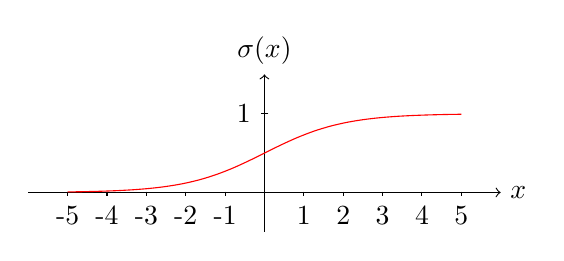
\begin{tikzpicture}
      \draw[->] (-3,0) -- (3,0) node[right]{$x$};
      \draw[->] (0,-0.5) -- (0,1.5) node[above]{$\sigma(x)$};
      \foreach \x in {-5,-4,-3,-2,-1,1,2,3,4,5}
        \draw (\x/2,0.01) -- (\x/2,-0.05) node[below] {\x};
      \foreach \y in {1}
        \draw (0.05,\y) -- (-0.05,\y) node[left] {\y};
      \draw[domain=-5:5,smooth,variable=\x,red] plot ({\x/2},{1/(1 + exp(-\x))});
    \end{tikzpicture}
    \captionof{figure}{Sigmoid funktionen i intervallet $x \in [-5, 5]$}
    \label{fig:sigmoid}
  \end{center}
\end{minipage}
Typisk har et neuralt netværk flere neuroner i hvert lag, og antallet af vægte og biases er derfor meget større. $x$, $y$, samt alle de forskellige $a_n$ og $b_n$ for hvert lag er søjlevektorer, og $w_n$ i alle lag er matricer. Derfor kan der bruges matrixmultiplikation for at kunne beregne outputtet. Dette er ikke et problem, da de pågældende regneoperationer er defineret tidligere.  
\newpage
\subsection{Træning af neurale netværk med Cross-Entropy}
Når et neuralt netværk initialiseres, er alle vægtene og biases tilfældige indenfor et interval. Dette betyder, at modellen ikke kan genkende noget, ligesom et barn, der skal lære noget for første gang. For at træne modellen til at genkende mønstre kræves et passende datasæt med labels, der angiver, hvad hvert input repræsenterer. For at kunne forbedre modellen skal vi måle, hvor god den er til at lave forudsigelser. I stedet for blot at måle antallet af korrekte gæt anvender man en såkaldt \textit{loss-funktion}, som kvantificerer, hvor præcist modellen forudsiger. For klassifikationsproblemer bruger man ofte \textit{cross-entropy loss}, som evaluerer forskellen mellem modellens sandsynlighedsfordeling og de faktiske labels. Loss-funktionen tager modellens sandsynligheder for hver klasse og beregner, hvor langt de er fra de korrekte labels. \parencite{sanderson2017neural,Sanderson_2017,Nielsen_2019b} Eksempelvis, hvis et datapunkt har en korrekt label i klasse 3, og modellen giver sandsynlighederne, her er $y_i$ modellens sandsynligheder og $\hat{y}_i$ den korrekte label:
\begin{align}
\mathbf{y}_i = \begin{bmatrix}
0.12 \\
0.03 \\
0.25 \\
0.07 \\
0.18 \\
0.09 \\
0.04 \\
0.11 \\
0.06 \\
0.05
\end{bmatrix}
&&
\hat{\mathbf{y}}_i = \begin{bmatrix}
0 \\
0 \\
1 \\
0 \\
0 \\
0 \\
0 \\
0 \\
0 \\
0
\end{bmatrix}
\end{align}
Cross-entropy loss beregnes ved formlen:
\begin{align}
L_i = -\sum_{j=1}^{10} \hat{y}_{ij} \log(y_{ij})
\end{align}
hvor $ \hat{y}_{ij} $ er den korrekte label, og $ y_{ij} $ er modellens forudsigelse for klasse $ j $. Dette sikrer, at modellen straffes hårdt for lave sandsynligheder på den korrekte klasse. Summen af loss over hele datasættet divideres med antallet af datapunkter for at få gennemsnitlig loss:
\begin{align}
L = \frac{1}{N} \sum_{i=1}^{N} L_i
\end{align}
Cross-entropy loss er kontinuert og differentierbar, hvilket gør det muligt at optimere ved hjælp af gradient descent. Målet er at minimere loss, så modellen bliver bedre til at forudsige. Dette gør cross-entropy til en standardmetode for klassifikationsopgaver, hvor sandsynlighedsfordelinger er i spil. \parencite{Kumar_2024,verma2020neuralnet}
\subsection{Over og underfitting}
To vigtige ting, man altid skal være opmærksom på, når man opstiller og træner neurale netværk, er \textit{overfitting} og \textit{underfitting}. Overfitting opstår, når modellen er for kompleks i forhold til træningsdataene, og derfor lærer modellen træningsdataene udenad og ikke kan generalisere denne viden til nye data. Underfitting opstår, når modellen er for simpel i forhold til træningsdataene og derfor ikke kan lære træningsdataene godt nok. Dette kan ses i træningsprocessen ved at sammenligne træningsnøjagtigheden med testnøjagtigheden. Hvis træningsnøjagtigheden er meget højere end testnøjagtigheden, er modellen overtilpasset, og hvis både træningsnøjagtigheden og testnøjagtigheden er lav, er modellen undertilpasset (eller datasættet er ikke generaliserbart). \parencite{Kirsanov_2024,sanderson2017neural}

\subsection{Softmax}
Softmax er en aktiveringsfunktion, der bruges i det sidste lag af et neuralt netværk, når outputtet skal repræsentere en sandsynlighedsfordeling over forskellige klasser. Softmax-funktionen tager en vektor af vilkårlige reelle tal og omdanner dem til en vektor af sandsynligheder, hvor summen af sandsynlighederne altid er lig 1. Softmax-funktionen er defineret som:
\begin{align}
  \text{softmax}(z_i) = \frac{e^{z_i}}{\sum_{j=1}^{K} e^{z_j}}
\end{align}
hvor $z_i$ er elementet i inputvektoren, og $K$ er antallet af klasser. \parencite{kurbiel2021softmax} Softmax-funktionen anvendes ofte i klassifikationsproblemer, hvor outputtet skal repræsentere sandsynligheden for hver klasse. Herunder ses et eksempel på softmax-funktionen anvendt på et enkelt datapunkt $i$:
\begin{align}
  \text{softmax}\left(\underbrace{\begin{bmatrix}
    2.0 \\
    1.0 \\
    0.1
  \end{bmatrix}}_{\text{Sum ikke lig 1}}\right)
  = \begin{bmatrix}
    \frac{e^{2.0}}{e^{2.0} + e^{1.0} + e^{0.1}} \\
    \frac{e^{1.0}}{e^{2.0} + e^{1.0} + e^{0.1}} \\
    \frac{e^{0.1}}{e^{2.0} + e^{1.0} + e^{0.1}}
  \end{bmatrix}
  = \underbrace{\begin{bmatrix}
    0.659 \\
    0.242 \\
    0.099
  \end{bmatrix}}_{\text{Sum lig 1}}
\end{align}
I dette eksempel er sandsynligheden for klasse 1 (første element) 65.9\%, for klasse 2 (andet element) 24.2\%, og for klasse 3 (tredje element) 9.9\%. Softmax-funktionen sikrer, at summen af sandsynlighederne er 1, hvilket gør det muligt at tolke outputtet som en sandsynlighedsfordeling. \parencite{Sanderson_2017}

\subsection{Gradient descent}
Gradient descent er en algoritme, der tager loss-funktionen og beregner gradienten af denne i forhold til alle modellens parametre (vægtene og biases). Gradienten er en vektor, der peger i retningen af den største stigning af loss-funktionen. For at minimere loss-funktionen bevæger vi os i den modsatte retning af gradienten. Dette gøres ved at opdatere vægtene og biases i modellen med gradienten ganget med en konstant, kaldet \textit{learning rate}. Processen gentages, indtil loss-funktionen er tilstrækkeligt minimeret. \parencite{IBM_2021, Sanderson_2017, Nielsen_2019a} Antag, at vi organiserer modellens vægte og biases i en søjlevektor $\vec{W}$, og at loss-funktionen er $L(\vec{W})$. Gradienten af loss-funktionen er $\nabla L(\vec{W})$. Derfor beskriver søjlevektoren $-\nabla L(\vec{W})$, hvordan vi kan opdatere $\vec{W}$ for at minimere loss-funktionen og dermed forbedre modellens præstation. Algoritmen, der finder gradienten på baggrund af modellens parametre og loss-funktionen, kaldes \textit{backpropagation}. \parencite{Sanderson_2017, Nielsen_2019a} Hvordan backpropagation fungerer, vil blive gennemgået mere detaljeret i et kommende afsnit. Indtil videre antager vi blot, at den fungerer som beskrevet og returnerer den korrekte gradient for modellens parametre.

\subsection{Partielle afledte}
Partielle afledte beskriver, hvordan en funktion ændrer sig, når én af dens variabler ændres, ved at de andre holdes konstante. Antag, vi har en funktion $f(x, y)$, der afhænger af to variabler $x$ og $y$. Den partielle afledte af $f$ med hensyn til $x$ betegnes $\frac{\partial f}{\partial x}$ og angiver hældningen af $f$ i $x$-retningen. Tilsvarende betegner $\frac{\partial f}{\partial y}$ hældningen i $y$-retningen. Partielle afledte er særligt nyttige i optimering af neurale netværk, hvor de spiller en central rolle i gradientbaserede algoritmer. Gradientens komponenter er netop de partielle afledte for hver variabel i modellen. Hvis vi eksempelvis ønsker at minimere en funktion $f(x, y)$, anvender vi gradienten $\nabla f(x, y)$, der består af $\frac{\partial f}{\partial x}$ og $\frac{\partial f}{\partial y}$, til effektivt at navigere mod lavere værdier af $f$. \parencite{Kirsanov_2024}

\subsection{Kædereglen}
Kædereglen er en fundamental regel i differentialregning, der gør det muligt at differentiere sammensatte funktioner. Hvis vi har to funktioner, $f(g(x))$, hvor $f$ afhænger af $g(x)$, og $g$ afhænger af $x$, siger kædereglen, at den afledte af $f$ med hensyn til $x$ er produktet af den afledte af $f$ med hensyn til $g$ og den afledte af $g$ med hensyn til $x$:
\begin{align}
  \frac{d}{dx} f(g(x)) = f'(g(x)) \cdot g'(x)
\end{align}
Med Leibniz notation kan kædereglen skrives som:
\begin{align}
  \frac{\partial f}{\partial x} = \frac{\partial f}{\partial z} \cdot \frac{\partial z}{\partial x}
  &&
  \text{hvor } z = g(x)
\end{align}
Kædereglen er en central del i neurale netværk og i machine learning, især i algoritmen backpropagation, hvor det kræves at beregne gradienten af en sammensat loss-funktion i forhold til modellens parametre. \parencite{Kirsanov_2024}
\subsection{Backpropagation}
Antag et simpelt neuralt netværk som det, der er vist i \figureref{fig:neural_network2} tidligere, og loss-funktionen for dette netværk, $L$. $L$ har som funktionsparameter alle modellens parametre og giver en kvantitativ vurdering af, hvor gode disse parametre er givet et datasæt. En primitiv måde at optimere modellens parametre på er at ændre hver parameter separat og undersøge, om loss-funktionen er højere eller lavere med de nye parametre. Hvis loss er lavere, ændres parameteren, hvis ikke, nulstilles parameteren, og den næste justeres. Gentages denne proces tilstrækkeligt mange gange, vil man nærme sig et lokalt minimum i loss-funktionen. Selvom denne metode er primitiv, kan den fungere for en simpel model som den, der er visualiseret i \figureref{fig:neural_network2}. Dog vil denne tilgang være ineffektiv og ekstremt langsom for en model med hundredevis eller tusindvis af parametre og er derfor ikke en praktisk metode for den gældende problemstilling. Denne vilkårlige permutationsalgoritme er den bedste metode i generelle tilfælde, da der ikke nødvendigvis findes en bedre metode. \parencite{Kirsanov_2024} For differentiable udregninger, som dem i et neuralt netværk, findes der dog en langt bedre metode, der muliggør markant mere effektiv optimering af modellens parametre. Denne algoritmes formål er at forudsige, hvordan en ændring i modellens parametre vil påvirke loss-funktionen, uden at justere manuelt. Selvom denne algoritme kan lyde umulig, bygger den faktisk på fundamentale matematiske principper. Algoritmen kaldes \textit{backpropagation}. Og helt simpelt går denne algoritme ud på at udregne gradienten af loss funktionen i forhold til alle modellens parametre, således at gradienten kan udregnes så medlelen kan effektivt optimeres. \parencite{Kirsanov_2024, Nielsen_2019b, Sanderson_2017} eksemplet herunder gennemgår hvordan de afledte udregnes i et simpelt neuralt netværk for at illustrere backpropagation anvendt.
\subsubsection{Udregning af gradienten}
Beskue det nedstående neurale netværk med 1 neuron i hvert lag og et skjult lag. Dette afsnit har til formål at gennemgå, hvordan gradienten af loss funktionen udregnes i forhold til vægtene og biases i modellen. Dette eksempel bruger sigmoid aktiveringsfunktionen og kvadratisk loss funktion, som er en lidt anden end den tidligere beskrevne cross-entropy loss funktion. Dette er gjort, da de partielle afledte er lettere at udregne i dette tilfælde og vil derfor gøre det lettere at forstå backpropagation.
\begin{center}
  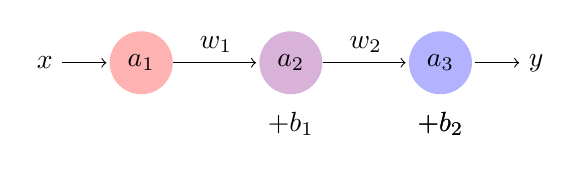
\begin{tikzpicture}
  \node[circle, minimum size=8mm, fill=red!30] (Input-1) at (0,0) {$a_1$};  % Input Layer
  \node[circle, minimum size=8mm, fill=violet!30] (Hidden-1) at (1.9,0) {$a_2$};  % Hidden Layer
  \node[below=0.1cm of Hidden-1] (Hidden-1-bias) {$+b_1$};
  \node[circle, minimum size=8mm, fill=blue!30] (Output-1) at (3.8,0) {$a_3$};  % Output Layer
  \node[below=0.1cm of Output-1] (Output-1-bias) {$+b_2$};
  \node[below=0.1cm of Output-1] {$+b_2$};
  \draw[->, shorten >=1pt] (Input-1) -- (Hidden-1) node[midway, above]{$w_1$};  % Connect neurons
  \draw[->, shorten >=1pt] (Hidden-1) -- (Output-1) node[midway, above]{$w_2$};  % Connect neurons
  \draw[<-, shorten <=1pt] (Input-1) -- ++(-1,0) node[left]{$x$};  % Inputs
  \draw[->, shorten <=1pt] (Output-1) -- ++(1,0) node[right]{$y$};  % Outputs
\end{tikzpicture}
  \captionof{figure}{Et simpelt neuralt netværk}
  \label{fig:neural_network3}
\end{center}
For at simplificere senere udregninger, er modellen konstrueret således at kun $a_2$ benytter sig af en aktiveringsfunktion $\sigma(x)$. Så for at udregne $y$ givet $x$ kan denne udregnes således:
\begin{align}
  y= \sigma(w_1 \cdot x + b_1) \cdot w_2 + b_2  
\end{align}
Og lavet om til en funktion $f(x)$:
\begin{align}
  f(w_1, b_1, w_2, b_2, x) = \sigma(w_1 \cdot x + b_1) \cdot w_2 + b_2
\end{align}
Og insættes i loss funktionen $L(y)$:
\begin{align}
  L&(y_i) &&= (y_i - \hat{y}_i)^2 && \text{hvor } \hat{y}_i \text{ er det rigtige svar for $i$ indeks}\\
  L&(f(w_1, b_1, w_2, b_2, x)) &&= L(\sigma(w_1 \cdot x + b_1) \cdot w_2 + b_2)
  \label{eq:full_loss}
\end{align}
Hvis vi nu har en loss funktion $L(y_i)$, der kvantificerer, hvor god modellen er til at prediktere, kan vi nu udregne gradienten af $L$ i forhold til $w_1$, $b_1$, $w_2$ og $b_2$. Dette gøres ved at bruge kædereglen til at udregne de partielle afledte af $L$ i forhold til $w_1$, $b_1$, $w_2$ og $b_2$. Skrivemåden $y_i$ erstattes hermed med $y$ da indekset ikke er vigtigt for resten af eksemplet. Først udregnes $\frac{\partial L}{\partial b_2}$\\
Her kan kædereglen bruges til at udregne $\frac{\partial L}{\partial b_2}$:
\begin{align}
  \frac{\partial L}{\partial b_2} = \frac{\partial L}{\partial y} \cdot \frac{\partial y}{\partial b_2}
\end{align}
Lad os først udregne $\frac{\partial L}{\partial y}$, som er den partielle afledte af $L$ i forhold til $y$, denne er relativt simpel at udregne, da $L$ blot kan differentieres på normal vis:
\begin{align}
  \frac{\partial L}{\partial y} = 2 \cdot (y - \hat{y}) = 2y - 2\hat{y}
\end{align}
Og $\frac{\partial y}{\partial b_2}$, som er den partielle afledte af $y$ i forhold til $b_2$, denne er også simpel at udregne, da resten antages at være konstant og derfor ender vi med:
\begin{align}
  \frac{\partial y}{\partial {\color{blue}b_2}} = 1 && L(\overbrace{\sigma(w_1 \cdot x + b_1) \cdot w_2 + {\color{blue}b_2} }^{y} )
\end{align}
Så $\frac{\partial L}{\partial b_2}$ kan nu udregnes:
\begin{align}
  \frac{\partial L}{\partial b_2} &= \frac{\partial L}{\partial y} \cdot \frac{\partial y}{\partial b_2} = \frac{\partial L}{\Ccancel[red]{\partial y}} \cdot \frac{\Ccancel[red]{\partial y}}{\partial b_2}\\
  &= (2y - 2\hat{y}) \cdot 1 = 2y - 2\hat{y} \quad\text{hvor}\quad y = \sigma(w_1 \cdot x + b_1) \cdot w_2 + b_2\\
  &= 2\cdot\sigma(w_1 \cdot x + b_1) \cdot w_2 + 2b_2 - 2\hat{y}
\end{align}
Nu er $\frac{\partial L}{\partial b_2}$ udregnet! Nu kan $\frac{\partial L}{\partial w_2}$ udregnes på samme måde, først opdeles $\frac{\partial L}{\partial w_2}$ efter kædereglen:
\begin{align}
  \frac{\partial L}{\partial w_2} = \frac{\partial L}{\partial y} \cdot \frac{\partial y}{\partial w_2}
\end{align}
Eftersom $\frac{\partial L}{\partial y}$ allerede er udregnet, kan vi nu udregne $\frac{\partial y}{\partial w_2}$, som er den partielle afledte af $y$ i forhold til $w_2$. Dette kan udregnes da $w_2$ kun afhænger af $\sigma(w_1 \cdot x + b_1)$ og da den er konstant i forhold til $w_2$, den partielle afledte er derfor lig $\sigma(w_1 \cdot x + b_1)$:
\begin{align}
  \frac{\partial y}{\partial {\color{blue}w_2}} = \sigma(w_1 \cdot x + b_1) && L(\overbrace{\sigma(w_1 \cdot x + b_1) \cdot {\color{blue}w_2} + b_2}^{y} )
\end{align}
Så $\frac{\partial L}{\partial w_2}$ kan nu udregnes:
\begin{align}
  \frac{\partial L}{\partial w_2} &= \frac{\partial L}{\partial y} \cdot \frac{\partial y}{\partial w_2} = \frac{\partial L}{\Ccancel[red]{\partial y}} \cdot \frac{\Ccancel[red]{\partial y}}{\partial w_2}\\
  &= (2y - 2\hat{y}) \cdot \sigma(w_1 \cdot x + b_1) \quad\text{hvor}\quad y = \sigma(w_1 \cdot x + b_1) \cdot w_2 + b_2\\
  &= 2\cdot(\sigma(w_1 \cdot x + b_1) \cdot w_2 + b_2 - \hat{y}) \cdot \sigma(w_1 \cdot x + b_1)
\end{align}
Nu er $\frac{\partial L}{\partial w_2}$ udregnet! Nu kan $\frac{\partial L}{\partial b_1}$ udregnes på samme måde, Dog er denne mere kompleks, da den er "dybere" i kæden, og derfor skal der bruges kædereglen flere gange. Først opdeles $\frac{\partial L}{\partial b_1}$ efter kædereglen:
\begin{align}
  \frac{\partial L}{\partial b_1} = \frac{\partial L}{\partial y} \cdot \frac{\partial y}{\partial a_2} \cdot \frac{\partial a_2}{\partial b_1}
\end{align}
Beskue \figureref{fig:neural_network3} og Ligning \eqref{eq:full_loss} for hvordan $a_2$ er defineret. Så $\frac{\partial L}{\partial b_1}$ kan nu udregnes, da $\frac{\partial L}{\partial y}$ allerede er udregnet, kan vi nu udregne $\frac{\partial y}{\partial a_2}$, som er den partielle afledte af $y$ i forhold til $a_2$. Her kan samme tankegang bruges idet $a_2$ kun afhænger af $w_2$:
\begin{align}
  \frac{\partial y}{\partial {\color{blue}a_2}} = w_2 && L(\overbrace{{\color{blue}\sigma(w_1 \cdot x + b_1)} \cdot w_2 + b_2}^{y} )
\end{align}
Nu kan $\frac{\partial a_2}{\partial b_1}$ udregnes, som er den partielle afledte af $a_2$ i forhold til $b_1$. Her vil den partielle afledte være $\sigma'(w_1 \cdot x + b_1)$, da $a_2$ afhænger direkte af $b_2$ gennem aktiveringsfunktionen
\begin{align}
  \frac{\partial a_2}{\partial {\color{blue}b_1}} = \sigma'(w_1 \cdot x + b_1) && L(\overbrace{\sigma(w_1 \cdot x + {\color{blue}b_1})}^{a_2} \cdot w_2 + b_2)
\end{align}
Så $\frac{\partial L}{\partial b_1}$ kan nu udregnes:
\begin{align}
  \frac{\partial L}{\partial b_1} &= \frac{\partial L}{\partial y} \cdot \frac{\partial y}{\partial a_2} \cdot \frac{\partial a_2}{\partial b_1} = \frac{\partial L}{\Ccancel[red]{\partial y}} \cdot \frac{\Ccancel[red]{\partial y}}{\Ccancel[red]{\partial a_2}} \cdot \frac{\Ccancel[red]{\partial a_2}}{\partial b_1}\\
  &= (2y - 2\hat{y}) \cdot w_2 \cdot \sigma'(w_1 \cdot x + b_1) \quad\text{hvor}\quad y = \sigma(w_1 \cdot x + b_1) \cdot w_2 + b_2\\
  &= 2\cdot(\sigma(w_1 \cdot x + b_1) \cdot w_2 + b_2 - \hat{y}) \cdot w_2 \cdot \sigma'(w_1 \cdot x + b_1)
\end{align}
Nu er $\frac{\partial L}{\partial b_1}$ udregnet! Nu kan $\frac{\partial L}{\partial w_1}$ udregnes på samme måde, På samme måde er denne mere kompleks, da den også er "dybere" i kæden, og derfor skal der bruges kædereglen flere gange. Først opdeles $\frac{\partial L}{\partial w_1}$ efter kædereglen:
\begin{align}
  \frac{\partial L}{\partial w_1} = \frac{\partial L}{\partial y} \cdot \frac{\partial y}{\partial a_2} \cdot \frac{\partial a_2}{\partial w_1}
\end{align}
Så $\frac{\partial L}{\partial w_1}$ kan nu udregnes, da $\frac{\partial L}{\partial y}$ og $\frac{\partial y}{\partial a_2}$ allerede er udregnet, Nu kan $\frac{\partial a_2}{\partial w_1}$ udregnes, som er den partielle afledte af $a_2$ i forhold til $w_1$. Da $a_2 = \sigma(w_1 \cdot x + b_1)$, afhænger $a_2$ af $w_1$ gennem argumentet, og med hensyn til kædereglen, vil den partielle afledte være:
\begin{align}
  \frac{\partial a_2}{\partial {\color{blue}w_1}} = x \cdot \sigma'(w_1 \cdot x + b_1) && L(\overbrace{\sigma({\color{blue}w_1} \cdot x + b_1)}^{a_2} \cdot w_2 + b_2 )
\end{align}
Så $\frac{\partial L}{\partial w_1}$ kan nu udregnes:
\begin{align}
  \frac{\partial L}{\partial w_1} &= \frac{\partial L}{\partial y} \cdot \frac{\partial y}{\partial a_2} \cdot \frac{\partial a_2}{\partial w_1} = \frac{\partial L}{\Ccancel[red]{\partial y}} \cdot \frac{\Ccancel[red]{\partial y}}{\Ccancel[red]{\partial a_2}} \cdot \frac{\Ccancel[red]{\partial a_2}}{\partial w_1}\\
  &= (2y - 2\hat{y}) \cdot w_2 \cdot x \cdot \sigma'(w_1 \cdot x + b_1) \quad\text{hvor}\quad y = \sigma(w_1 \cdot x + b_1) \cdot w_2 + b_2\\
  &= 2\cdot(\sigma(w_1 \cdot x + b_1) \cdot w_2 + b_2 - \hat{y}) \cdot w_2 \cdot x \cdot \sigma'(w_1 \cdot x + b_1)
\end{align}
Lad os tage et skridt tilbage og opsummere, hvad der er blevet udregnet. Vi har nu udregnet gradienten af loss funktionen i forhold til modellens parametre, netop $w_1$, $b_1$, $w_2$ og $b_2$. Dette er essentielt for at kunne træne modellen effektivt, da vi nu ved, hvordan loss funktionen ændrer sig, når vi ændrer vægtene og biases. Dette gør det muligt at bruge gradient descent til at minimere loss funktionen og dermed forbedre modellens præstation. Dette gøres i priksis ved at gemme aktiveringerne af de forskellige lag når modellen prediktere, og derefter bruge disse mellemregninger til at regne baglæns og dermed finde gradienten, det er her algoritmen backpropagation får sit navn. Selvom eksemplet i dette afsnit er simpelt, kan samme principper anvendes på langt mere komplekse neurale netværk med mange flere lag og neuroner. Her vil værdierne dog være matricer og vektorer, og derfor vil de partielle afledte således også være organiseret i matricer, mens dette lyder komplekst, er det i praksis blot en udvidelse af de principper, der er blevet gennemgået i dette afsnit, bare med flere indekser.\\\\
Lad os for en god ordens skyld tjekke vores svar efter ved brug af Maple CAS værktøjet:
\begin{align}
  &L(y)\coloneqq(y-\hat{y})^{2}\colon\\
  &f(w_{1},b_{1},w_{2},b_{2},x)\coloneqq\sigma(w_{1}\cdot x+b_{1})\cdot w_{2}+b_{2}\colon\\
  &\frac{\partial L}{\partial b_{2}}=\text{diff}(L(f(w_{1},b_{1},w_{2},b_{2},x)),b_2)=\color{blue}2\cdot\sigma(w_{1}\cdot x+b_{1})\cdot w_{2}+2\cdot b_{2}-2\cdot\hat{y}\\
  &\frac{\partial L}{\partial w_{2}}= \text{diff}(L(f(w_{1},b_{1},w_{2},b_{2},x)),w_2)=\color{blue}2\cdot(\sigma(w_{1}\cdot x+b_{1})\cdot w_{2}+b_{2}-\hat{y})\cdot\sigma(w_{1}\cdot x+b_{1})\\
  &\frac{\partial L}{\partial b_{1}}= \text{diff}(L(f(w_{1},b_{1},w_{2},b_{2},x)),b_1)=\color{blue}2\cdot(\sigma(w_{1}\cdot x+b_{1})\cdot w_{2}+b_{2}-\hat{y})\cdot w_{2}\cdot\sigma'(w_{1}\cdot x+b_{1})\\
  &\frac{\partial L}{\partial w_{1}}= \text{diff}(L(f(w_{1},b_{1},w_{2},b_{2},x)),w_1)=\color{blue}2\cdot(\sigma(w_{1}\cdot x+b_{1})\cdot w_{2}+b_{2}-\hat{y})\cdot w_{2}\cdot x\cdot\sigma'(w_{1}\cdot x+b_{1})
\end{align}
Som det ses er vores svar korrekt, og dermed er vores udregninger korrekte. Da udledningen af de afledte for at mere kompliceret netværk ikke er meget anderledes end hvad der tidligere er gennemgået, vil de afledte fra \parencite{keita2023backpropagation,verma2020neuralnet,kurbiel2021softmax} såvel som den samme generelle tankegang blive brugt til at udlede de partielle afledte uden dybere redegørelse, da dette ligger langt over opgavens omfang/niveau.
\section{Valg af programmeringssprog}
Til at implementere et neuralt netværk, er det nødvændigt at vælge et programmeringssprog, der er egnet til formålet. Der findes mange forskellige programmeringssprog, der kan bruges til at implementere neurale netværk, herunder Python, R, Java, C++, og mange flere. Men da det ønskes at programmet er interaktivt og let at bruge, er Python med PyGame eller Java med Processing de mest oplagte valg. Python og mere specifikt NumPy, som er et bibliotek til Python, er enormt brugervenligt og hurtigt at udføre matriceregning i. Java er også et godt valg, da det er et meget populært programmeringssprog, med faste typer som gør det nemmere at undgå fejl. Processing er et bibliotek til Java, der gør det nemt at lave grafik og interaktive applikationer. Men grundet Python's kompakte syntaks, er det valgt til udviklingen af programmet.
\section{Neuralt netværk implementeret i Python}
Til genkendelse af håndskrevne tal anvendes MNIST-datasættet, som er et velkendt benchmark inden for maskinlæring. Datasættet indeholder billeder af håndskrevne tal med opløsning på $28\times28$ pixels skal input laget have $28\cdot28=748$ inputs. til de skjulte lag blev der nogenlunde arbitrært valgt 2 lag af 16 neuroner, outputlaget er bestående af 10 neuroner hvor hver repræsenterer sandsynligheden for at inputtet er det givne tal. Der blev valgt at bruge sigmoid funktionen som aktiveringsfunktion i de skjulte lag og softmax i outputlaget. Der blev valgt at bruge loss funktionen \textit{cross-entropy loss} da det er en standard loss funktion til klassifikationsopgaver. Og gradient decent algorimen bruges til at minimere loss funktionen.
\subsection{Dataindlæsning}
MNIST datasættet er meget populært og der ligger derfor allerede en masse implementeringer af indlæsning af datasættet på nettet. Der blev valgt at bruge en implementering fra \parencite{Khodabakhsh} da den er udviklet som en klasse og derfor er nem at bruge. Klassen er vist i \listingref{lst:mnist_dataloader} i bilag, og kan indlæse både trænings- og testdatasættet med metoden \texttt{load\_data()}. denne process tager ca. 1000ms på en almindelig computer, og skal kun køres en gang, når programmet starter, da dataen gemmes i arbejdshukommelsen efterfølgende. 

\subsection{Tegnefladen}
%Tegnefladen som ses på \listingref{lst:run} på linje 26-87
Da opgaveformuleringen kræver et "tegneprogram", hvori brugeren selv kan indtaste tal, vil netop dette udvikles. Her tages Python med biblioteket PyGame i brug, da det tilbyder en række funktioner til at tegne til et vindue på computeren. Først skal et vindue laves:
\inputminted[firstline=8, lastline=11]{python}{run.py}\noindent
Nu er vinduet tegnet. Det blev valgt at lave tegnefladen som en klasse. Klassen skal holde styr på opløsningen såvel som alle pixelsene. Derfor kan vi definere konstruktøren således:
\inputminted[firstline=26, lastline=34]{python}{run.py}\noindent
Her er \texttt{self.dx} og \texttt{self.dy} opløsningen af tegnefladen. \texttt{self.pixel\_size} er størrelsen af pixelsene. Da pixelsene altid bør være kvadratiske, tages \texttt{min()} af både den lodrette og vandrette dimension. \texttt{self.pixel\_values} er værdierne af alle de forskellige pixels i et 2D-array. Alle værdierne starter som 0. \texttt{self.last\_pixel\_x} og \texttt{self.last\_pixel\_y} er interne variable til at holde styr på tegnelogikken. Dette forklares senere. Nu kan tegnefladen tegnes til vinduet:
\inputminted[firstline=62, lastline=74]{python}{run.py}\noindent
Denne kode tegner et gitter af rektangler på skærmen ved at iterere gennem \texttt{self.dx} og \texttt{self.dy} og bruger \texttt{pygame.draw.rect} til at tegne hvert rektangel med en farve baseret på \texttt{self.pixel\_values}, såvel som en grå 1-pixel-tyk border. For at opdatere tegnefladen, når brugeren tegner med musen, blev metoden \texttt{handle\_event()} udviklet:
\inputminted[firstline=36, lastline=60]{python}{run.py}\noindent
\texttt{handle\_event()} tjekker først, om hændelsen er \texttt{pygame.MOUSEBUTTONDOWN}. Hvis ikke, afsluttes funktionen. Musens klik-koordinater konverteres til gitterkoordinater på tegnefladen og sammenlignes med det sidste klik for at sikre, at den kun opdaterer én gang per pixel. Hvis gitterkoordinaterne er gyldige, opdaterer funktionen den seneste klikposition (\texttt{self.last\_pixel\_x} og \texttt{self.last\_pixel\_y}) og justerer pixelværdierne i en 3x3-rude omkring klikket. For hver nabocelle beregnes afstanden til musen. En ny pixelværdi (maks. 255) beregnes og opdateres, hvis den nye værdi er højere end den nuværende. Herunder på \figureref{fig:drawingpad} ses et eksempel på dette, hvor den røde streg er den faktiske sti, som musen tog. Yderligere kan hele tegnefladeklassen beskues i \listingref{lst:run} på linje 26-87:
\begin{center}
  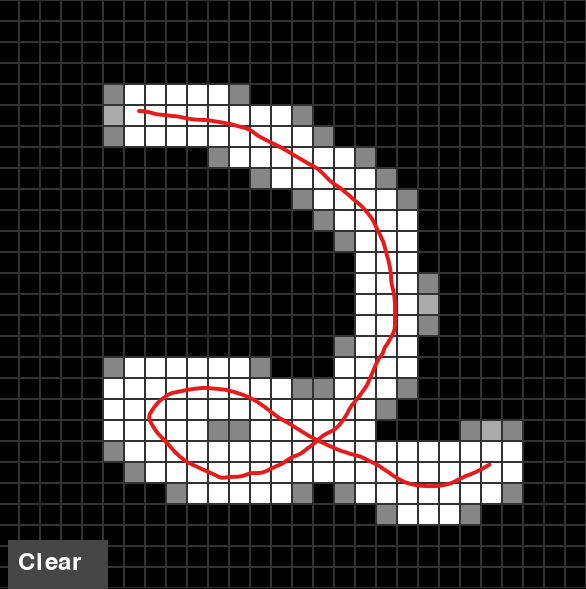
\includegraphics[width=0.5\textwidth]{drawingpad.png}
  \captionof{figure}{Eksempel på tegnefladen og den faktiske sti, som musen tog}
  \label{fig:drawingpad}
\end{center}
Som ses på billedet muliggør afstandsmetoden at tegne en mere realistisk sti hvor der opstår et naturligt gradient i intensiteten. denne metode er valgt da den imiterer MNIST-datasættets udseende bedre end en simpel binær metode, og siden modellen er trænet på MNIST-datasættet, vil det give bedre resultater at komme så tæt på datasættet som muligt. 
\subsection{Prediktering}
Hver frame opdateres modellens prediktion af det tegnede tal. Til dette bruges metoden \texttt{predict()}, den bruger modellens parametre som er gemt i \texttt{model.npz} filen, herunder ses indlæsningen af disse parametre samt selve \texttt{predict()} metoden:
\inputminted[firstline=100, lastline=110]{python}{run.py}\noindent
\inputminted[firstline=89, lastline=97]{python}{run.py}\noindent
\texttt{.npz} formatet er blot et format til at gemme flere NumPy arrays i en fil. i \texttt{main()} metoden indlæses disse parametre og gemmes i variablerne \texttt{w1}, \texttt{b1}, \texttt{w2}, \texttt{b2}, \texttt{w3} og \texttt{b3}. Disse bruges i \texttt{predict()} metoden sammen med et input, som er en 2D-array af pixelværdierne, som bliver lavet om til \texttt{x} med \texttt{.reshape(-1)}, hvor hver række er sat sammen til en lang række. Herunder ses selve \texttt{predict()} metoden bare skrevet som matematik:
\begin{align}
  y = \operatorname{softmax}\left( W_3 \cdot \sigma\left( W_2 \cdot \sigma\left( W_1 \cdot X + B_1 \right) + B_2 \right) + B_3 \right)
\end{align}
Denne ligning repræsenterer outputtet $y$ fra \texttt{predict()}. Modellen udfører følgende beregninger: Inputtet $X$ multipliceres med vægtmatricen $W_1$ og lægges sammen med biasvektoren $B_1$. Resultatet \texttt{Z1} gennemgår sigmoid aktiveringsfunktionen $\sigma$. Denne proces gentages for det andet lag med vægte $W_2$ og bias $B_2$. I det tredje lag multipliceres de transformerede data med $W_3$, lægges sammen med $B_3$, og sendes gennem softmax-funktionen. Til sidst anvendes en cross-entropy loss funktionen $L$ på outputtet. Operatoren $\cdot$ betegner matrixmultiplikation, hvilket er passende i denne sammenhæng, dog er samme operator i Python-notation lig \texttt{@}. i koden er \texttt{Z} blot en betegnelse for værdierne i de forskellige lag før de sendes gennem aktiveringsfunktionen og bliver til \texttt{A}. Så for at prediktere modellen med værdierne fra tegnefladen kan man gøre således:
\inputminted[firstline=133, lastline=134]{python}{run.py}\noindent
\subsection{De afledte}
Som tidligere beskrevet er selve udregningen af de partielle afledte over opgavens omfang og vil derfor ikke blive udregnet fra bunden. Der vil tages udgangspunkt i de afledte fra \parencite{keita2023backpropagation,verma2020neuralnet,kurbiel2021softmax}. De afledte nævnt i disse kilder antages at være korrekte, dog vil de senere blive testet med \textit{finite difference} metoden for at sikre deres korrekthed. \parencite{verma2020neuralnet} påstår følgende afledte for de forskellige lag i et netværk med 1 skjult lag med Cross-Entropy loss og Softmax aktiveringsfunktion i outputlaget:
\begin{align}
  dZ_2 &= \frac{\partial L}{\partial Z_2} = A_2 - Y\\
  dW_2 &= \frac{\partial L}{\partial W_2} = \frac{1}{m}(dZ_2 \cdot A_1^T)\\
  dB_2 &= \frac{\partial L}{\partial B_2} = \frac{1}{m}\sum dZ_2\\
  dZ_1 &= \frac{\partial L}{\partial Z_1} = W_2^T \cdot \sigma'(Z_1)\\
  dW_1 &= \frac{\partial L}{\partial W_1} = \frac{1}{m}(dZ_1 \cdot X^T)\\
  dB_1 &= \frac{\partial L}{\partial B_1} = \frac{1}{m}\sum dZ_1
\end{align}
Hvor $m$ er antallet af træningsdata, $A_1$ og $A_2$ er aktiveringerne i de forskellige lag, $Y$ er de rigtige svar, og $\sigma'$ er den afledte af sigmoid funktionen, bemærk at $Z$ er værdierne i de forskellige lag før de sendes gennem aktiveringsfunktionen og hermed bliver til $A$. Kilden \parencite{kurbiel2021softmax} er enige med denne differentiering af Cross-entry loss og Softmax aktiveringsfunktionen. Da vores model er bestående af 2 skjulte lag, kan disse afledte udvides til at gælde for 2 skjulte lag, da hver lag kun er afhængig af det forrige, er det blot en udvidelse af de samme principper som tidligere beskrevet ba begge de skjulte lag er aktiveret med sigmoid funktionen. Derfor kan de afledte for hele modellen skrives som:
\begin{align}
  dZ_3 &= \frac{\partial L}{\partial Z_3} = A_3 - Y\\
  dW_3 &= \frac{\partial L}{\partial W_3} = \frac{1}{m}(dZ_3 \cdot A_2^T)\\
  dB_3 &= \frac{\partial L}{\partial B_3} = \frac{1}{m}\sum dZ_3\\
  dZ_2 &= \frac{\partial L}{\partial Z_2} = W_3^T \cdot \sigma'(Z_2)\\
  dW_2 &= \frac{\partial L}{\partial W_2} = \frac{1}{m}(dZ_2 \cdot A_1^T)\\
  dB_2 &= \frac{\partial L}{\partial B_2} = \frac{1}{m}\sum dZ_2\\
  dZ_1 &= \frac{\partial L}{\partial Z_1} = W_2^T \cdot \sigma'(Z_1)\\
  dW_1 &= \frac{\partial L}{\partial W_1} = \frac{1}{m}(dZ_1 \cdot X^T)\\
  dB_1 &= \frac{\partial L}{\partial B_1} = \frac{1}{m}\sum dZ_1
\end{align}
Bemærk her hvordan $dZ_2$, $dW_2$ og $dB_2$ på samme måde som $dZ_1$, $dW_1$ og $dB_1$ da de på lige vis kun er afhængige af det forrige lags værdier. Disse afledte kan nu implementeres i Python således:
\inputminted[firstline=43, lastline=61]{python}{train.py}\noindent
Bemærk på linje 55-60 hvordan indlæringsraten ganges med gradienten og subtraheres fra vægtene og biases. Dette er selve gradient descent algoritmen, som bruges til at minimere loss funktionen. Bemærk også at de afledte bruger den afledte af sigmoid funktionen, hvor i koden bruges \texttt{sigmoid\_derivative\_from\_sigmoid\_output(y)} frem for \texttt{sigmoid\_derivative(x)} til at udregne denne. Beskue \listingref{lst:activations} i bilag for at se implementeringen af denne funktion, Men grunden til dette er at sigmoid funktionen allerede er udregnet i \texttt{predict()} metoden tidligere, og derfor kan den bruges til at udregne hældningen meget hurtigere end hvis den skulle udregnes igen. Det kan også tydligt ses at \texttt{sigmoid\_derivative\_from\_sigmoid\_output(y)} er hurtigere end \texttt{sigmoid\_derivative(x)} i \listingref{lst:activations} i bilag på linje 6-11. Selvom det er en lille besparelse enkeltvis, vil denne funktion blive kaldt enormt mange gange, og derfor er det vigtigt at den er så hurtig som muligt, så man undgår at udregne ting flere gange, når det ikke er nødvendigt. \parencite{smith2024sigmoid}
\subsection{Træning}
På baggrund af de implementerede metoder kan modellen nu trænes. Dette gøres i \texttt{train()} metoden, som ses herunder:
\inputminted[firstline=63, lastline=80]{python}{train.py}\noindent
\texttt{train()} er konstrueret således, at den træner modellen over et specificeret antal epochs. For hver epoch bliver træningsdataene blandet med en tilfældig permutation af indeks, der genereres med \texttt{np.random.permutation(X.shape[0])}. Herefter omorganiseres \texttt{X} og \texttt{Y} baseret på denne rækkefølge for at sikre, at træningsforløbet ikke bliver påvirket af dataenes oprindelige rækkefølge. Efter blandingen opdeles de blandede data i mindre batches af 1.000 datapunkter hver. Dette muliggør brugen af mini-batch gradient descent, som er en mere effektiv, men støjende tilgang til minimering af loss-funktionen, da den bruger en tilnærmelse af gradienten. Dette har som biprodukt, at den kan undslippe visse lokale minima. For hvert batch kaldes først \texttt{predict()}-metoden, som beregner modellens prediktioner, og derefter \texttt{update()}-metoden, som opdaterer modellens parametre med backpropagation-algoritmen. Hver 10. epoch evalueres og logges modellen ydeevne, både på træningsdataene og på et separat testdatasæt, som består af 10.000 datapunkter, der ikke er blevet brugt til træning. Dette gøres for at overvåge modellens præstation på nye, usete data, såvel som for at undgå overfitting. For at gemme modellen bliver den løbende gemt i en fil kaldet \texttt{model.npz} hver 100. epoch ved hjælp af \texttt{export\_to\_file()}-metoden, som kalder \texttt{np.savez()}-metoden fra NumPy. Dette giver mulighed for at stoppe træningen, når et tilfredsstillende resultat er opnået. Samlet set implementerer \texttt{train()} en standard træningsproces for et neuralt netværk, som inkluderer datablanding, mini-batch-træning, løbende evaluering og lagring af modellen.\\\\
Når denne metode kaldes ses følgende i konsollen:
\begin{minted}{console}
  C:/.../sop> python train.py
  Loading MNIST data...
  MNIST data loaded.
  Epoch 10 Loss: 0.3930, Accuracy: 88.67%, Test Accuracy: 88.72%
  Epoch 20 Loss: 0.2989, Accuracy: 91.32%, Test Accuracy: 91.01%
  Epoch 30 Loss: 0.2545, Accuracy: 92.58%, Test Accuracy: 92.12%
  Epoch 40 Loss: 0.2264, Accuracy: 93.43%, Test Accuracy: 92.66%
  Epoch 50 Loss: 0.2062, Accuracy: 94.03%, Test Accuracy: 93.15%
  Epoch 60 Loss: 0.1910, Accuracy: 94.46%, Test Accuracy: 93.53%
  Epoch 70 Loss: 0.1792, Accuracy: 94.84%, Test Accuracy: 93.85%
  Epoch 80 Loss: 0.1694, Accuracy: 95.09%, Test Accuracy: 94.07%
  Epoch 90 Loss: 0.1610, Accuracy: 95.33%, Test Accuracy: 94.25%
  Epoch 100 Loss: 0.1536, Accuracy: 95.54%, Test Accuracy: 94.31%
\end{minted}
Med denne model arkitektur på 2 skjulte lag med 16 neuroner i hvert er en testnøjagtighed på 94.31\% efter 100 epochs yderst fyldestgørende til denne opgaves brugstilfælde. Dette resultat er opnået med en træningstid på ca. 40 sekunder på en almindelig computer. Yderligere epochs forbedre ikke medellen markant og derfor er det ikke nødvendigt at træne modellen længere. Hvordan modellen kan forbedres yderligere vil blive diskuteret i et senere afsnit.
\subsection{Genkendelse af brugerinput}
Når modellen er trænet, kan den bruges til at genkende brugerinput. De vigtige dele af denne rutine er allerede præsenteret tidligere, se \listingref{lst:run} for hele rutinen. Når brugeren tegner et tal på tegnefladen, opdateres modellens prediktioner i realtid. Denne metode er effektiv nok til at tidstagning på metoden ikke er relevant, på en almindelig computer er denne metode hurtig nok til at kunne køre hver frame uden problemer. Herunder ses programmet i aktion:
\begin{center}
  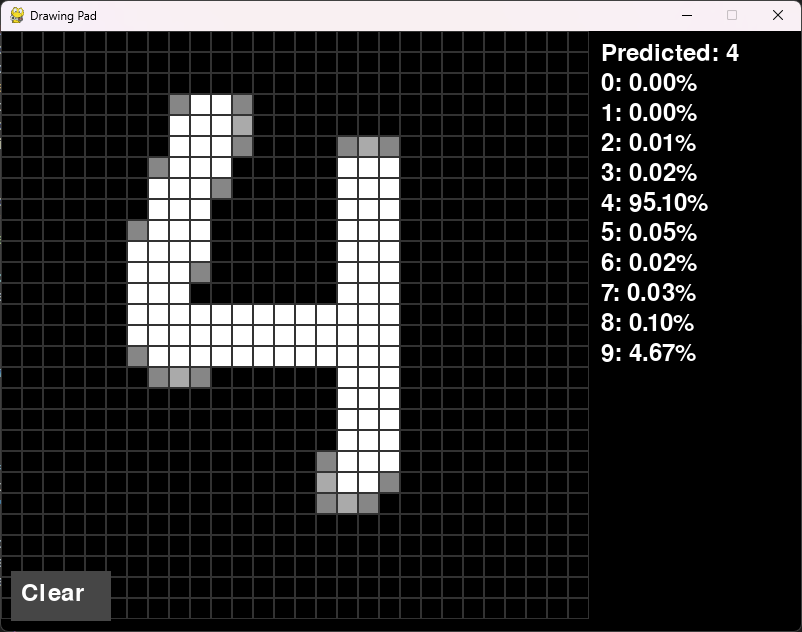
\includegraphics[width=0.5\textwidth]{drawingpad2.png}
  \captionof{figure}{Tegnefladen i aktion}
  \label{fig:drawingpad2}
\end{center}
På \figureref{fig:drawingpad2} ses tegnefladen i aktion, hvor brugeren har tegnet et 4-tal som modellen aldrig har set før. Modellen har dog ingen problemer med at genkende tallet som et 4-tal med overvejende sikkerhed. Dette er et godt tegn på at modellen er generaliseret og ikke overtilpasset til træningsdataene.
\section{Vurdering af neurale netværk til genkendelse af håndskrevne tal}
% snak om test og train accuracy OK
% denne data er ikke nødvendigvis repræsentativ for virkelighedes brugstilfælde
% center of mass shift i datasættet
% data augmentation
Som ses i træningsprocessen, er modellen trænet til en testnøjagtighed på 94.31\% efter 100 epochs. I virkeligheden, med udgangspunkt i brugerens input, vil denne nøjagtighed være lavere. Grunden til dette er, at MNIST-datasættet er centreret med \textit{center of mass}-algoritmen, som er en algoritme, der finder centrum af "massen" i et billede og translaterer billedet, således at centrum af massen er i midten af billedet. Derudover er datasættet også skaleret, således at der hverken er meget små eller meget store tal i datasættet størrelsesmæssigt. Dette er ikke tilfældet med brugerinput, som kan være skaleret og translateret på mange forskellige måder, som modellen ikke har lært at håndtere. Derfor vil modellen have en lavere nøjagtighed på brugerinput end på testdatasættet. Der er to måder uden om denne begrænsning: Den ene er at bruge data augmentation, som er en teknik, hvor man tilføjer støj som rotering, skalering og tilfældige pixels til træningsdatasættet for at gøre modellen mere robust overfor forskellige inputs. Den anden måde er at udføre samme preprocesseringsalgoritme, som datasættet har gennemgået, på brugerinputtet. Dette vil fjerne variansen i brugerinputtet og øge nøjagtigheden.\\\\
% overfitting - træning med for mange parametre
% underfitting - træning med for få parametre
Den trænede model er i dette tilfælde hverken overtilpasset eller undertilpasset da det ses at træningsnøjagtigheden og testnøjagtigheden meget tæt på hinanden i dette tilfælde, hvilket er et godt tegn på, at modellen er generaliseret og ikke overtilpasset. Dette kan også verificeres ved at afprøve modellen på egne tegninger, som tidligere beskrevet. Det blev nævnt, at valget af 2 lag af 16 neuroner var nogenlunde arbitrært, og derfor kan det være interessant at undersøge, hvordan modellen præsterer med flere eller færre neuroner i de skjulte lag, såvel som flere eller færre lag. Dette er en kunst i sig selv og kræver en masse eksperimentering og erfaring for at finde den optimale modelarkitektur. Man kan dog overbevise sig selv om, at det første skjulte lag finder de mindre detaljer i billedet, såsom hjørner og kurver, mens det andet skjulte lag finder de større detaljer, som cirkler og linjer. Dette kulminerer i outputlaget, som tager disse detaljer og bruger dem til at genkende tallet. \parencite{Sanderson_2017} Dette er blot et gæt på, hvordan denne maskine tænker. I virkeligheden er det relativt komplekst at undersøge, hvordan modellen reelt "tænker," da ingen har fortalt den, hvordan den skal genkende tal, modellens adfærd er fremspirende som funktion af datasættet.\\\\
% testing af de afledte med finite difference 
% hvordan kan modellen forbedres - generaliseres yderligere
% EVT: dropout
\subsection{Validering af de afledte ved at teste gradienten med finite difference}
\begin{wrapfigure}{r}{6cm}
  \vspace{-0.5cm}
  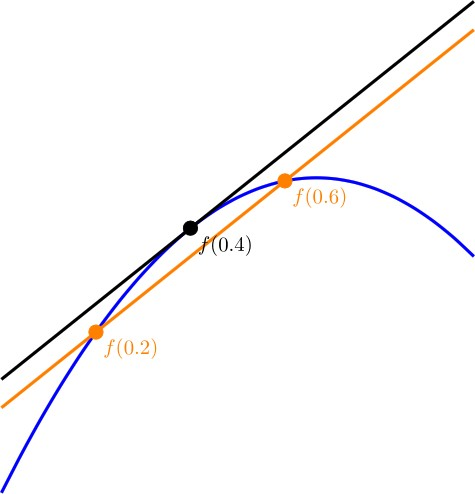
\includegraphics[width=6cm]{fd.jpg}
  \vspace{-0.8cm}
  \caption{Finite difference metoden fra \parencite{pranckevicius2015finite}}
  \label{fig:fd}
\end{wrapfigure}
Som nævnt tidligere er de afledte for det fulde netværk ikke blevet udregnet fra bunden, men derimod delvist taget fra internetkilder, mens resten er blevet regnet manuelt. Selvom beviset for disse ligger uden for opgavens niveau, er det stadig kritisk at teste disse afledte for at sikre deres korrekthed. Dette gøres ved brug af \textit{finite difference}-metoden, som er en metode til at estimere gradienten af en funktion ved at tage forskellen mellem to punkter, der er meget tæt på hinanden. Dette kan ses på \figureref{fig:fd}. Denne metode er meget simpel og kræver ikke differentialregning for at udføre. Metoden indebærer at tage to punkter med samme afstand fra $x$. Disse punkter er $x-\epsilon$ og $x+\epsilon$, hvor $\epsilon$ er en meget lille værdi. Nu kan gradienten estimeres som:
\begin{align}
  \frac{f(x+\epsilon)-f(x-\epsilon)}{2\epsilon}\approx f'(x)
\end{align}
Værdien $\epsilon$ vil i teorien være så lille som muligt, da dette vil øge nøjagtigheden af estimatet. Dog er man typisk begrænset af maskinens præcision. Datatypen \texttt{float} har en præcision på ca. 6-9 decimaltal \parencite{wagner2022floating}, og derfor vil det være fordelagtigt at vælge $\epsilon$ i en størrelsesorden, så man ikke mister præcision. I dette tilfælde er $\epsilon=10^{-4}$ valgt. Når man arbejder med neurale netværk, som grundlæggende er funktioner af mange variable, kan denne metode bruges til at estimere gradienten. Det gøres ved at tilføje en lille permutation til hver parameter i modellen, én ad gangen, og udføre beregningen for hver af dem. Ved at gentage dette for alle parametrene i modellen kan man sammenligne de estimerede gradienter med de gradienter, som modellen har beregnet. Hvis de to sæt gradienter stemmer godt overens, er de beregnede gradienter korrekte. Den endelige implementering af denne metode kan ses i \listingref{lst:train} på linje 85-128. Når metoden køres, ses følgende i konsollen:
\begin{minted}{console}
  C:/.../sop> python train.py
  Loading MNIST data...
  MNIST data loaded.
  Gradient check for W1: min = 0.0000000000, max = 0.0000664145, mean = 0.0000001361
  Gradient check for b1: min = 0.0000000080, max = 0.0000002913, mean = 0.0000001115
  Gradient check for W2: min = 0.0000000060, max = 0.0000352297, mean = 0.0000004651
  Gradient check for b2: min = 0.0000000940, max = 0.0000019676, mean = 0.0000003838
  Gradient check for W3: min = 0.0000000684, max = 0.0000012608, mean = 0.0000001779
  Gradient check for b3: min = 0.0000000890, max = 0.0000003139, mean = 0.0000001627
  Gradient check execution time: 1.9709 seconds
\end{minted}
Som det ses, er de estimerede gradienter meget tæt på de udregnede gradienter for alle parametrene i modellen. Dog er \texttt{W1}- og \texttt{W2}-gradienterne højere end de andre. Dette skyldes primært, at disse værdier er mere indviklede at udregne, og derfor er der en øget chance for, at usikkerhed ophober sig i værdierne. Dette er dog ikke et problem, da alle forskellende i de 2 udregninger er meget tæt på 0. Derfor kan det konkluderes, at de udregnede gradienter er korrekte, og dermed er de afledte nu vist at være korrekte.
% begrensninger af vanilla nn
% andre typer af nn og hvilke fordele de har (CNN)
\subsection{Begrænsninger af et simpelt neuralt netværk}
Selvom et simpelt neuralt netværk som det, der er implementeret i denne opgave, er vist til at være effektivt til genkendelse af håndskrevne tal i realtid, er der stadig begrænsninger og ulemper ved denne tilgang. En af de største begrænsninger ved simple neurale netværk er, at positionen af det tegnede tal på tegnefladen har stor betydning for modellens prediktering. Hvis et 2-tal tegnes i midten, har modellen typisk ingen problemer med at genkende tallet, hvorimod hvis samme 2-tal tegnes i hjørnet af tegnefladen, vil modellen sandsynligvis prediktere forkert. I simple neurale netværk kigges der på hele billedet som en lang række af pixels, som ikke er sammenhængende. Dette er ikke optimalt, idet håndskrevne tal typisk er sammenhængende, og derfor vil det være fordelagtigt at kigge på sammenhængen mellem pixels. Dette kan gøres med et Convolutional Neural Network (CNN). Et CNN er en type neuralt netværk, som er specielt designet til at lede efter mønstre i data. Denne type modeller har specialiserede lag, der kaldes convolutional lag, som er i stand til at finde mønstre i nærtliggende data ved at træne på mønstre i små dele af dataen. Dette gør CNN'er meget effektive til at genkende mønstre i data som billeder, lyd og tekst. Fordi positionen af det tegnede tal på tegnefladen ikke vil have nogen særlig betydning for modellens prediktering, vil en CNN-model være mere robust overfor forskellige inputs i dette brugstilfælde. Med deres mere komplekse arkitektur medfølger dog også en øget træningsbyrde og øget kompleksitet i udledningen af resultaterne. Dette er grunden til, at et simpelt neuralt netværk er valgt til denne opgave. Men CNN'er er vist til at yde markant bedre på MNIST-datasættet. En variant af CNN'er ydede en testnøjagtighed på 99.7\% på MNIST-datasættet \parencite{LeCun_1994}, og derfor vil det være nyttigt at bruge en CNN-model eller en anden mere kompleks model til at genkende håndskrevne tal i en reel applikation.

\newpage
\section{Konklusion}
I denne opgave er der blevet udviklet et neuralt netværk til genkendelse af håndskrevne tal i realtid uden brug af unødvændige abstraktioner i Python. der blev redegjort for neurale netværk såvel som de grundlæggende matematiske principper bag neurale netværk, herunder matrixmultiplikation og kædereglen. Modellen er bestående af 2 skjulte lag med 16 neuroner i hvert lag med sigmoid aktiveringsfunktioner og et outputlag med softmax aktiveringsfunktion. Modellen er trænet på MNIST-datasættet og opnåede en testnøjagtighed på 94.31\% efter 100 epochs. Modellens parametre blev vurderet kvantitativt ved at bruge cross-entropy loss funktionen. For at sikre nøjagtigheden af modellens gradienter blev finite difference metoden anvendt, hvilket bekræftede de udregnede gradienters korrekthed. Begrænsningerne ved det simple neurale netværk blev også diskuteret, især modellens følsomhed overfor positionen af håndskrevne tal. Det blev bemærket, at mere komplekse modeller som Convolutional Neural Networks (CNN'er) kan overvinde disse begrænsninger og forbedre modellens ydeevne markant. Alt i alt viser denne opgave, at selv et simpelt neuralt netværk kan opnå høj nøjagtighed i genkendelse af håndskrevne tal, men der er stadig plads til forbedringer som f.eks. at anvende mere avancerede modeltyper.
\newpage
\addcontentsline{toc}{section}{Literatur}
\printbibliography

\newpage
\addcontentsline{toc}{section}{Bilag}
\section*{Bilag}
\subsection*{mnist\_dataloader.py}
\begin{code}
  \inputminted{python}{mnist_dataloader.py}
  \caption{Python kode til indlæsning af MNIST datasættet}
  \label{lst:mnist_dataloader}
\end{code}
\newpage

\subsection*{activations.py}
\begin{code}
  \inputminted{python}{activations.py}
  \caption{Python kode til aktiveringsfunktioner}
  \label{lst:activations}
\end{code}
\newpage

\subsection*{train.py}
\begin{code}
  \inputminted{python}{train.py}
  \caption{Python kode til træning af neuralt netværk}
  \label{lst:train}
\end{code}
\newpage

\subsection*{run.py}
\begin{code}
  \inputminted{python}{run.py}
  \caption{Python kode til kørsel af neuralt netværk}
  \label{lst:run}
\end{code}

\end{document}